%===================================================================================
% Chapter: Introduction
%===================================================================================
\chapter{Desarrollo de la propuesta}\label{chapter:desarrollo}
%===================================================================================
El primer paso en nuestro proyecto fue la descarga del dataset de imágenes desde el servidor.

Se realizó una investigación exhaustiva sobre el estado del arte en el campo de procesamiento de imágenes para generación de textos alternativos. El resumen incluyó una caracterización de las formas de aprendizaje en los modelos de Machine Learning, la arquitectura que se llevó a cabo para el desarrollo del algoritmo, el modelo de lenguaje empleado, así como los datasets y métricas que fueron seleccionados durante el entrenamiento y evaluación de los modelos. 

Se seleccionaron los modelos que mejor se adaptaban a nuestro caso, optando por BLIP y Visual Transformers (GPT-2), los cuales destacan por su eficacia en tareas de procesamiento de imágenes y generación de texto. 

Se realizó un análisis exploratorio de los datos para comprender mejor las características y peculiaridades del dataset, lo cual contribuyó a identificar patrones y posibles problemas que podrían ser enfrentados durante el procesamiento de las imágenes.

Se procesaron todas las imágenes localmente utilizando los modelos seleccionados y mediante el uso de CLIP, se seleccionó la descripción que mejor se adaptaba a cada imagen.

Utilizamos las métricas BLEU y METEOR sobre los resultados obtenidos para evaluar el rendimiento de nuestros modelos, lo que nos permitió medir la efectividad de nuestro enfoque.

Finalmente, analizamos estadísticas básicas sobre los resultados finales. Este análisis nos proporcionó una visión clara de la calidad y consistencia de nuestras descripciones generadas y nos ayudó a identificar áreas de mejora para futuros proyectos.

\begin{figure}
	\centering
	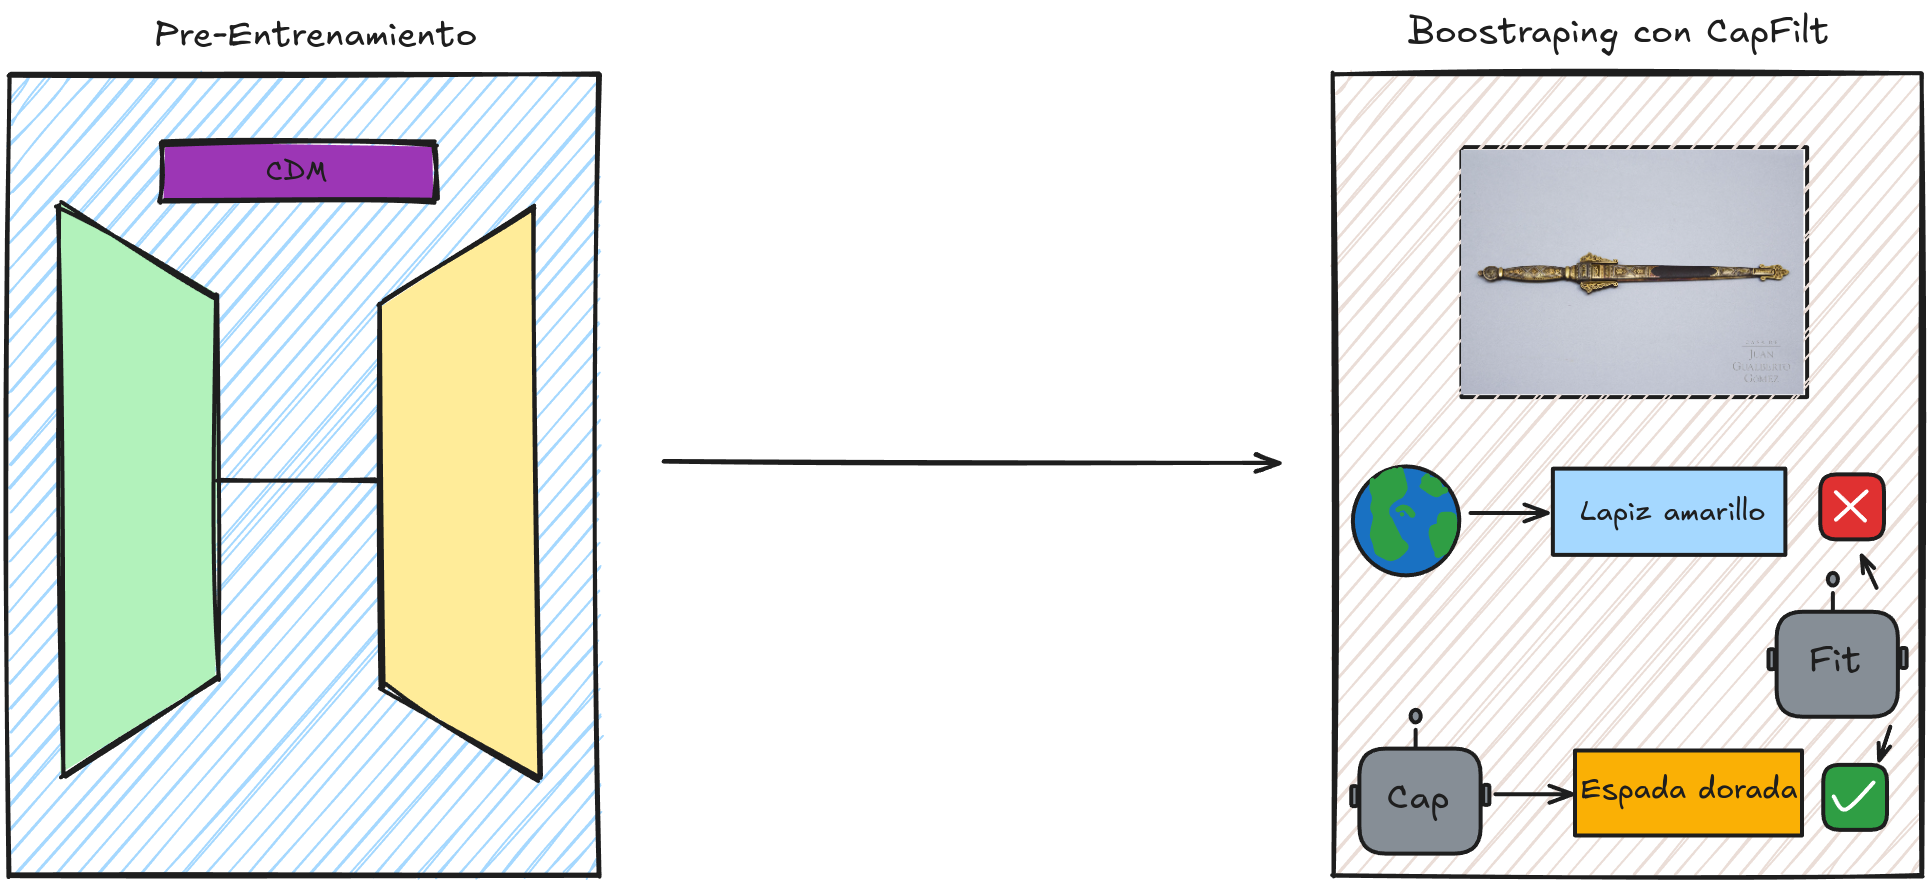
\includegraphics[width=1\linewidth]{Graphics/BLIP}
	\caption{}
	\label{fig:blip}
\end{figure}
\begin{figure}
	\centering
	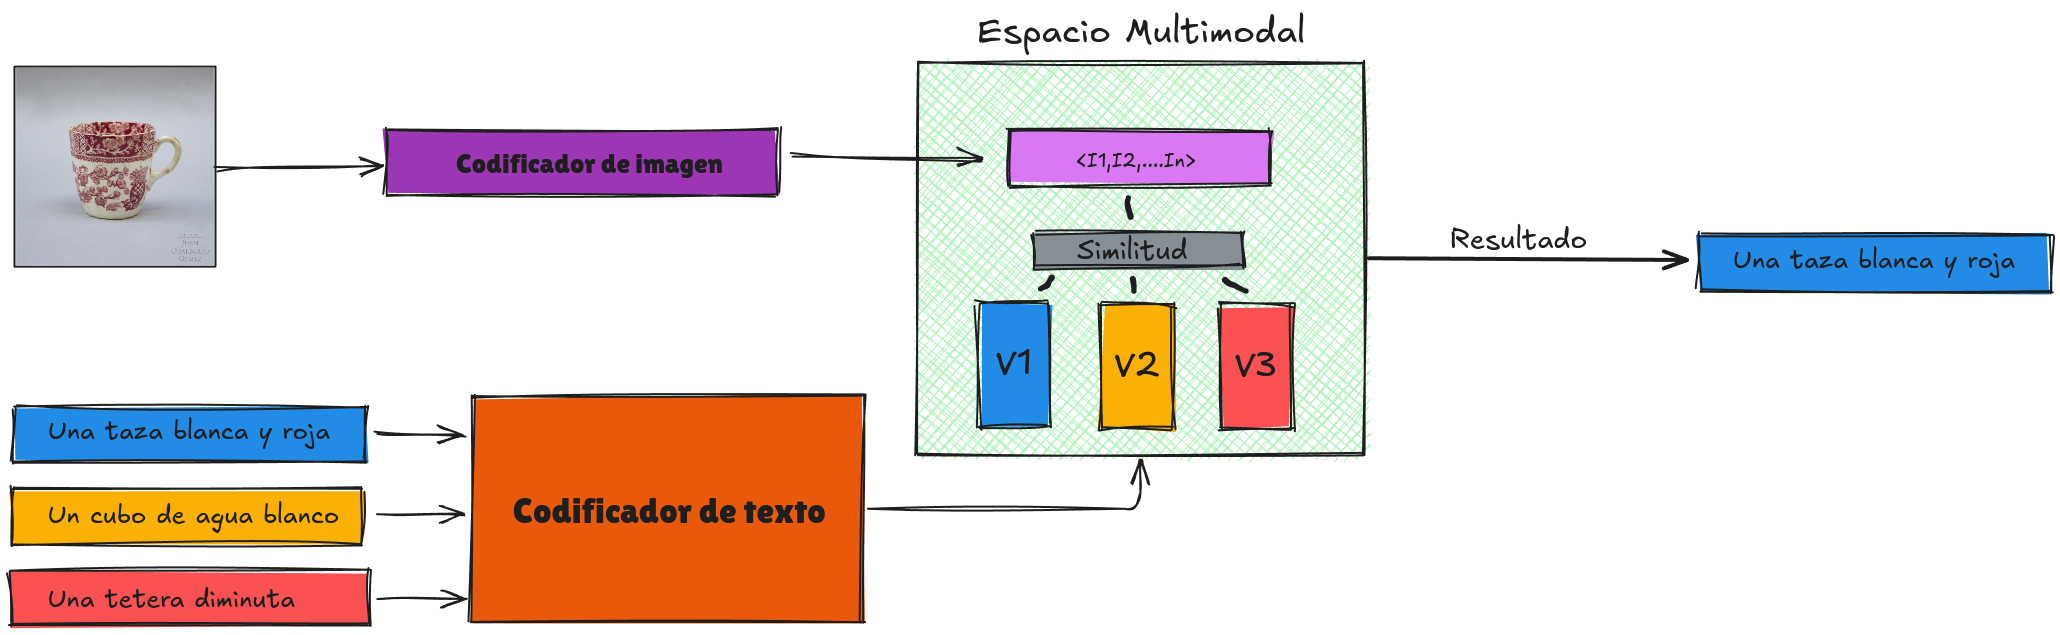
\includegraphics[width=1\linewidth]{Graphics/run_clip}
	\caption{}
	\label{fig:runclip}
\end{figure}
\begin{figure}
	\centering
	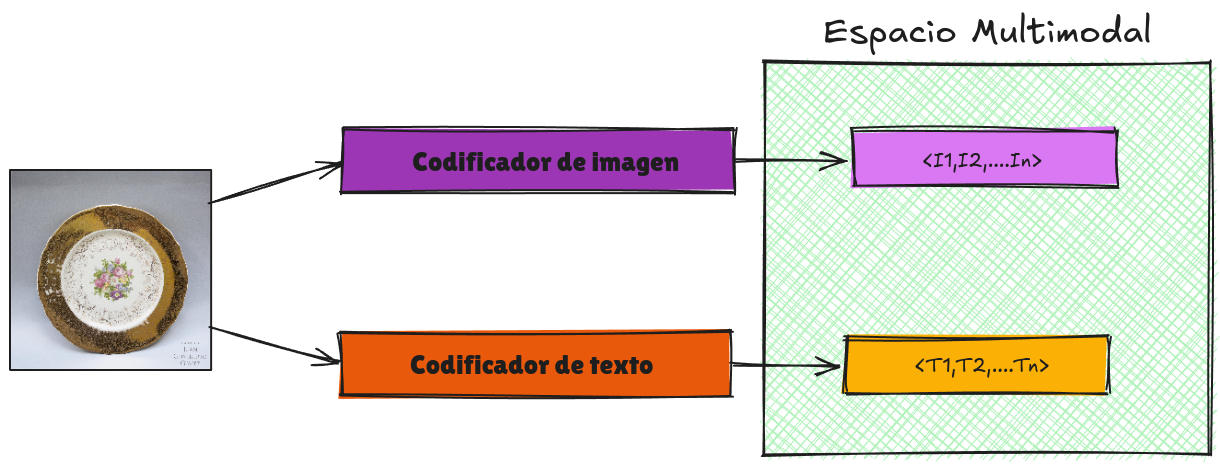
\includegraphics[width=1\linewidth]{Graphics/train_clip}
	\caption{}
	\label{fig:trainclip}
\end{figure}
\begin{figure}
	\centering
	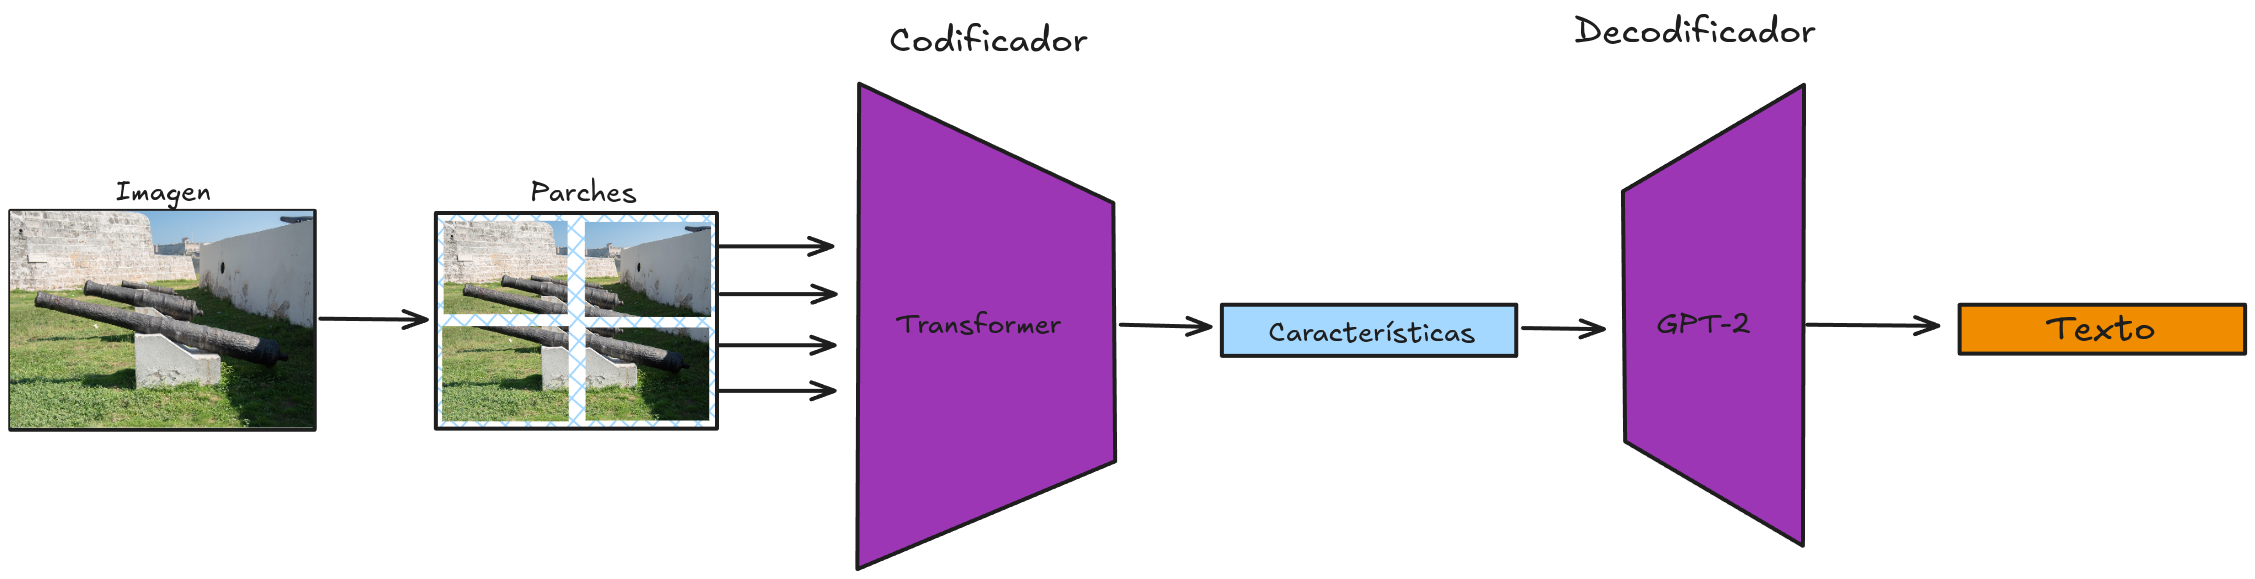
\includegraphics[width=1\linewidth]{Graphics/ViT}
	\caption{}
	\label{fig:vit}
\end{figure}
